\documentclass[a4paper,12pt]{article}
\usepackage{amsmath,amssymb,amsfonts,amsthm}
\usepackage{tikz}
\usepackage[utf8x]{inputenc}
\usepackage[T2A]{fontenc} 
\usepackage[russian]{babel}
\usepackage{cmap} 
\usepackage{ gensymb }
% Так ссылки в PDF будут активны
\usepackage[unicode]{hyperref}
\usepackage{ textcomp }
\usepackage{indentfirst}
\usepackage[version=3]{mhchem}

% вы сможете вставлять картинки командой \includegraphics[width=0.7\textwidth]{ИМЯ ФАЙЛА}
% получается подключать, как минимум, файлы .pdf, .jpg, .png.
\usepackage{graphicx}
% Если вы хотите явно указать поля:
\usepackage[margin=1in]{geometry}
% Или если вы хотите задать поля менее явно (чем больше DIV, тем больше места под текст):
% \usepackage[DIV=10]{typearea}

\usepackage{fancyhdr}

\newcommand{\bbR}{\mathbb R}%теперь вместо длинной команды \mathbb R (множество вещественных чисел) можно писать короткую запись \bbR. Вместо \bbR вы можете вписать любую строчку букв, которая начинается с '\'.
\newcommand{\eps}{\varepsilon}
\newcommand{\bbN}{\mathbb N}
\newcommand{\dif}{\mathrm{d}}

\newtheorem{Def}{Определение}


\pagestyle{fancy}
\makeatletter % сделать "@" "буквой", а не "спецсимволом" - можно использовать "служебные" команды, содержащие @ в названии
\fancyhead[L]{\footnotesize Квантовая физика}%Это будет написано вверху страницы слева
\fancyhead[R]{\footnotesize ФМХФ МФТИ}
\fancyfoot[L]{\footnotesize \@author}%имя автора будет написано внизу страницы слева
\fancyfoot[R]{\thepage}%номер страницы —- внизу справа
\fancyfoot[C]{}%по центру внизу страницы пусто

\renewcommand{\maketitle}{%
	\noindent{\bfseries\scshape\large\@title\ \mdseries\upshape}\par
	\noindent {\large\itshape\@author}
	\vskip 2ex}
\makeatother
\def\dd#1#2{\frac{\partial#1}{\partial#2}}


\title{4.2 \\ Исследование энергетического спектра $\beta$-частиц и определение их максимальной энергии при помощи магнитного спектрометра}
\author{Егор Берсенев} 
\date{16 февраля 2017 г.}

\begin{document}
	
	\maketitle
	\section{Теоретическое введение}
		Бета-распад это самопроизвольное преваращение ядер, при котором их массовове число не изменяется, а заряд изменяется на единицу. В данной работе мы будем иметь дело с электронным распадом:
		\begin{equation}
		    _{Z}^{A}X \rightarrow _{Z+1}^{A}X + e^{-} + \widetilde{\nu}
		\end{equation}
		Освобождающаяся в результате распада энергия делится между исходным ядром, электроном и нейтрино. При этом доля энергии, уносимая ядром крайне мала, так что вся энергия делится между нейтрино и электроном. Поэтому электроны могут иметь любую энергию от нулевой до некоторой макимальной энергии, высвобождаемой при распаде.
		
		Вероятность $\dif\omega$ того, что электрон вылетит с имульсом $\dif^3p$, а нейтрино с импульсом $\dif^3k$ равна произведению этих дифференциалов, но мы должны учесть также закон сохранения энергии.
		\begin{equation}
		    E_e - E - ck = 0
		\end{equation}
		Энергия электрона связана с импульсом обычным образом:
		\begin{equation}
		    E = c\sqrt{p^2 + m^2c^2} -mc^2
		\end{equation}
		Таким образом, вероятность $\dif\omega$ принимает вид:
		\begin{equation}
		    \dif\omega = D\delta(E_e-E-ck)\dif^3p\dif^3k = D\delta(E_e-E-ck)p^2\dif pk^2\dif k\dif\Omega_e\dif\Omega_{\widetilde{\nu}}
		\end{equation}
		D можно считать с хорошей точностью константой. В этом случае можно проинтегрировать по всем углам и по абсолютному значению импульса нейтрино. В этом случае $\delta$-функция исчезнет, а $ck$ всюду заменится на $E_e-E$. После умножения на полное число распадов выражение примет вид:
		\begin{equation}
		    \dif N = \frac{16\pi^2N_0}{c^2} D p^2\left(E_e-E\right)^2\dif p
		\end{equation}
		В нерелятивистском случае выражение упрощается и принимает вид:
		\begin{equation}
			\frac{\dif N}{\dif E} \simeq \sqrt{E}(E_e - E)^2
		\end{equation} 
		\begin{figure}[h!]
			\centering
			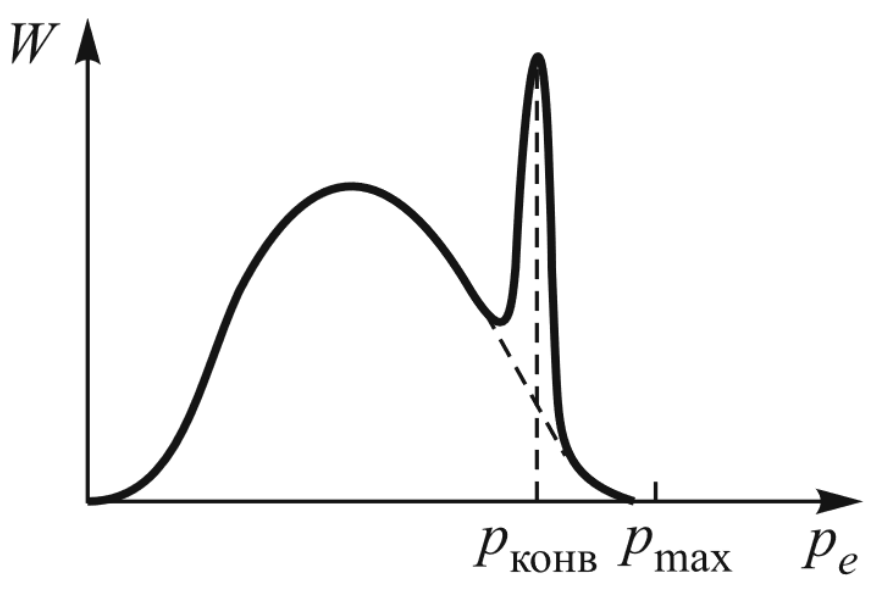
\includegraphics[width=0.6\linewidth]{pic1}
			\caption{Форма спектра $\beta$-частиц при разрешенных переходах}
		\end{figure}
		\section{Экспериментальная установка}
		Энергия определяется с помощью $\beta$-спектрометров. В работе используется магнитный спектрометр с короткой линзой.
		\begin{figure}
			\centering
			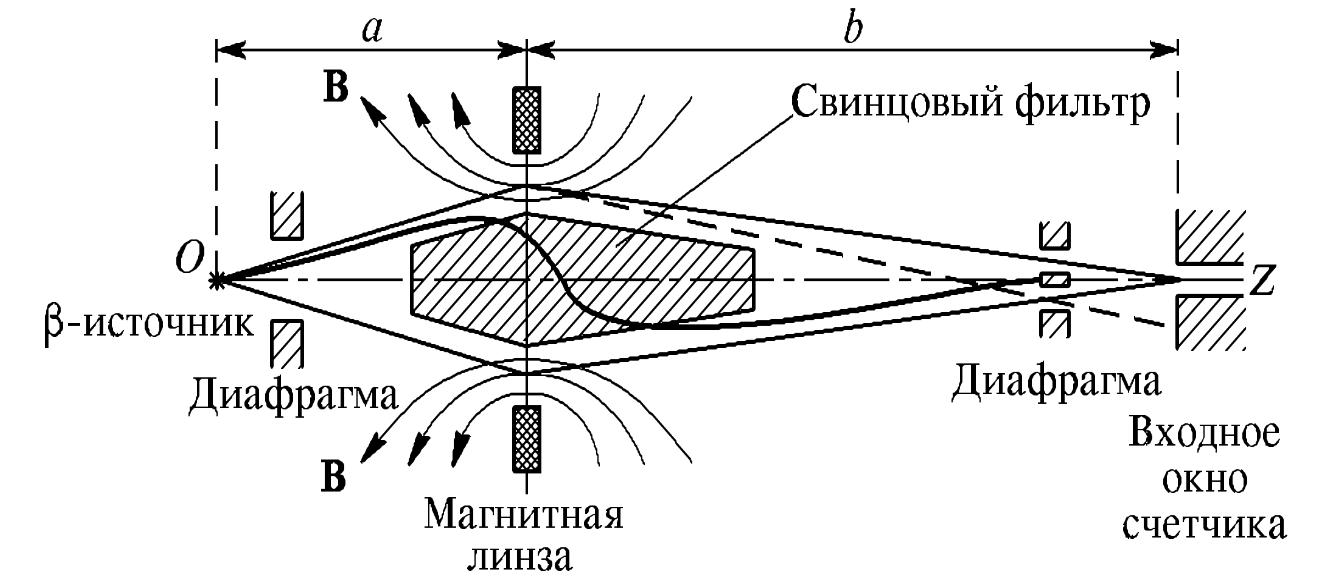
\includegraphics[width=0.8\linewidth]{pic2}
			\caption{Схема $\beta$-спектрометра с короткой линзой}
		\end{figure}
		Как показывает расчет, для заряженных частиц тонкая катушка эквивалентна линзе:
		\begin{equation}
			\frac{1}{f} \simeq \frac{I^2}{p_e^2}
		\end{equation}
		При заданной силе тока на входное окно счетчика собираются электроны с определенным импульсом.

    \section{Экспериментальные данные}
    Снимем точки $\beta$-спектра. Фоновое излучение равно $N_b = 0.775$. C учетом этого пересчитаем число частиц, зарегистрированных счетчиком.
    
    \begin{table}[h!]
\centering
\caption{Экспериментальные данные}
\label{my-label}
\begin{tabular}{|l|l|l|l|l|l|}
\hline
$I, A$    & $N, 1/s$   & $N-N_b, 1/s$ & $p, kEv/s$       & $E, kEv$      & $\frac{\sqrt{N}}{p}$ \\ \hline
0    & 0.85  & 0.0752  & 0.00    & 0      & ---     \\ \hline
0.2  & 0.78  & 0.0052  & 49.53   & 2.40   & 206.88  \\ \hline
0.5  & 0.94  & 0.1652  & 123.82  & 14.82  & 294.99  \\ \hline
0.7  & 0.94  & 0.1652  & 173.35  & 28.66  & 178.08  \\ \hline
0.9  & 1.26  & 0.4852  & 222.88  & 46.58  & 209.34  \\ \hline
1.1  & 1.919 & 1.1442  & 272.41  & 68.19  & 237.91  \\ \hline
1.3  & 2.279 & 1.5042  & 321.94  & 93.11  & 212.32  \\ \hline
1.5  & 2.969 & 2.1942  & 371.47  & 120.94 & 206.90  \\ \hline
1.7  & 3.399 & 2.6242  & 421.00  & 151.32 & 187.53  \\ \hline
1.9  & 3.929 & 3.1542  & 470.53  & 183.90 & 174.01  \\ \hline
2.1  & 4.079 & 3.3042  & 520.06  & 218.39 & 153.27  \\ \hline
2.3  & 4.739 & 3.9642  & 569.58  & 254.54 & 146.47  \\ \hline
2.5  & 4.479 & 3.7042  & 619.11  & 292.12 & 124.94  \\ \hline
2.7  & 4.339 & 3.5642  & 668.64  & 330.94 & 109.19  \\ \hline
2.9  & 3.469 & 2.6942  & 718.17  & 370.84 & 85.28   \\ \hline
3.1  & 2.799 & 2.0242  & 767.70  & 411.66 & 66.89   \\ \hline
3.3  & 2.019 & 1.2442  & 817.23  & 453.31 & 47.75   \\ \hline
3.5  & 1.55  & 0.7752  & 866.76  & 495.67 & 34.50   \\ \hline
3.7  & 0.98  & 0.2052  & 916.29  & 538.66 & 16.33   \\ \hline
3.9  & 2.769 & 1.9942  & 965.82  & 582.20 & 47.05   \\ \hline
4.1  & 5.198 & 4.4232  & 1015.35 & 626.23 & 65.00   \\ \hline
4.12 & 5.118 & 4.3432  & 1020.30 & 630.66 & 63.95   \\ \hline
4.15 & 5.198 & 4.4232  & 1027.73 & 637.31 & 63.83   \\ \hline
4.19 & 5.208 & 4.4332  & 1037.64 & 646.19 & 62.99   \\ \hline
4.22 & 5.258 & 4.4832  & 1045.06 & 652.87 & 62.67   \\ \hline
4.31 & 3.719 & 2.9442  & 1067.35 & 672.94 & 49.21   \\ \hline
4.38 & 2.329 & 1.5542  & 1084.69 & 688.60 & 34.90   \\ \hline
4.43 & 1.659 & 0.8842  & 1097.07 & 699.82 & 25.88   \\ \hline
4.58 & 0.43  & -0.3448 & 1134.22 & 733.60 & ---     \\ \hline
4.73 & 0.59  & -0.1848 & 1171.36 & 767.57 & ---     \\ \hline
4    & 5.428 & 4.6532  & 990.58  & 604.16 & 69.19   \\ \hline
3.95 & 4.429 & 3.6542  & 978.20  & 593.17 & 62.48   \\ \hline
3.8  & 1.13  & 0.3552  & 941.05  & 560.37 & 20.65   \\ \hline
3.85 & 1.57  & 0.7952  & 953.44  & 571.27 & 30.29   \\ \hline
\end{tabular}
\end{table}

\newpage

Построим график Ферми-Кюри.

\begin{figure}[h!]
			\centering
			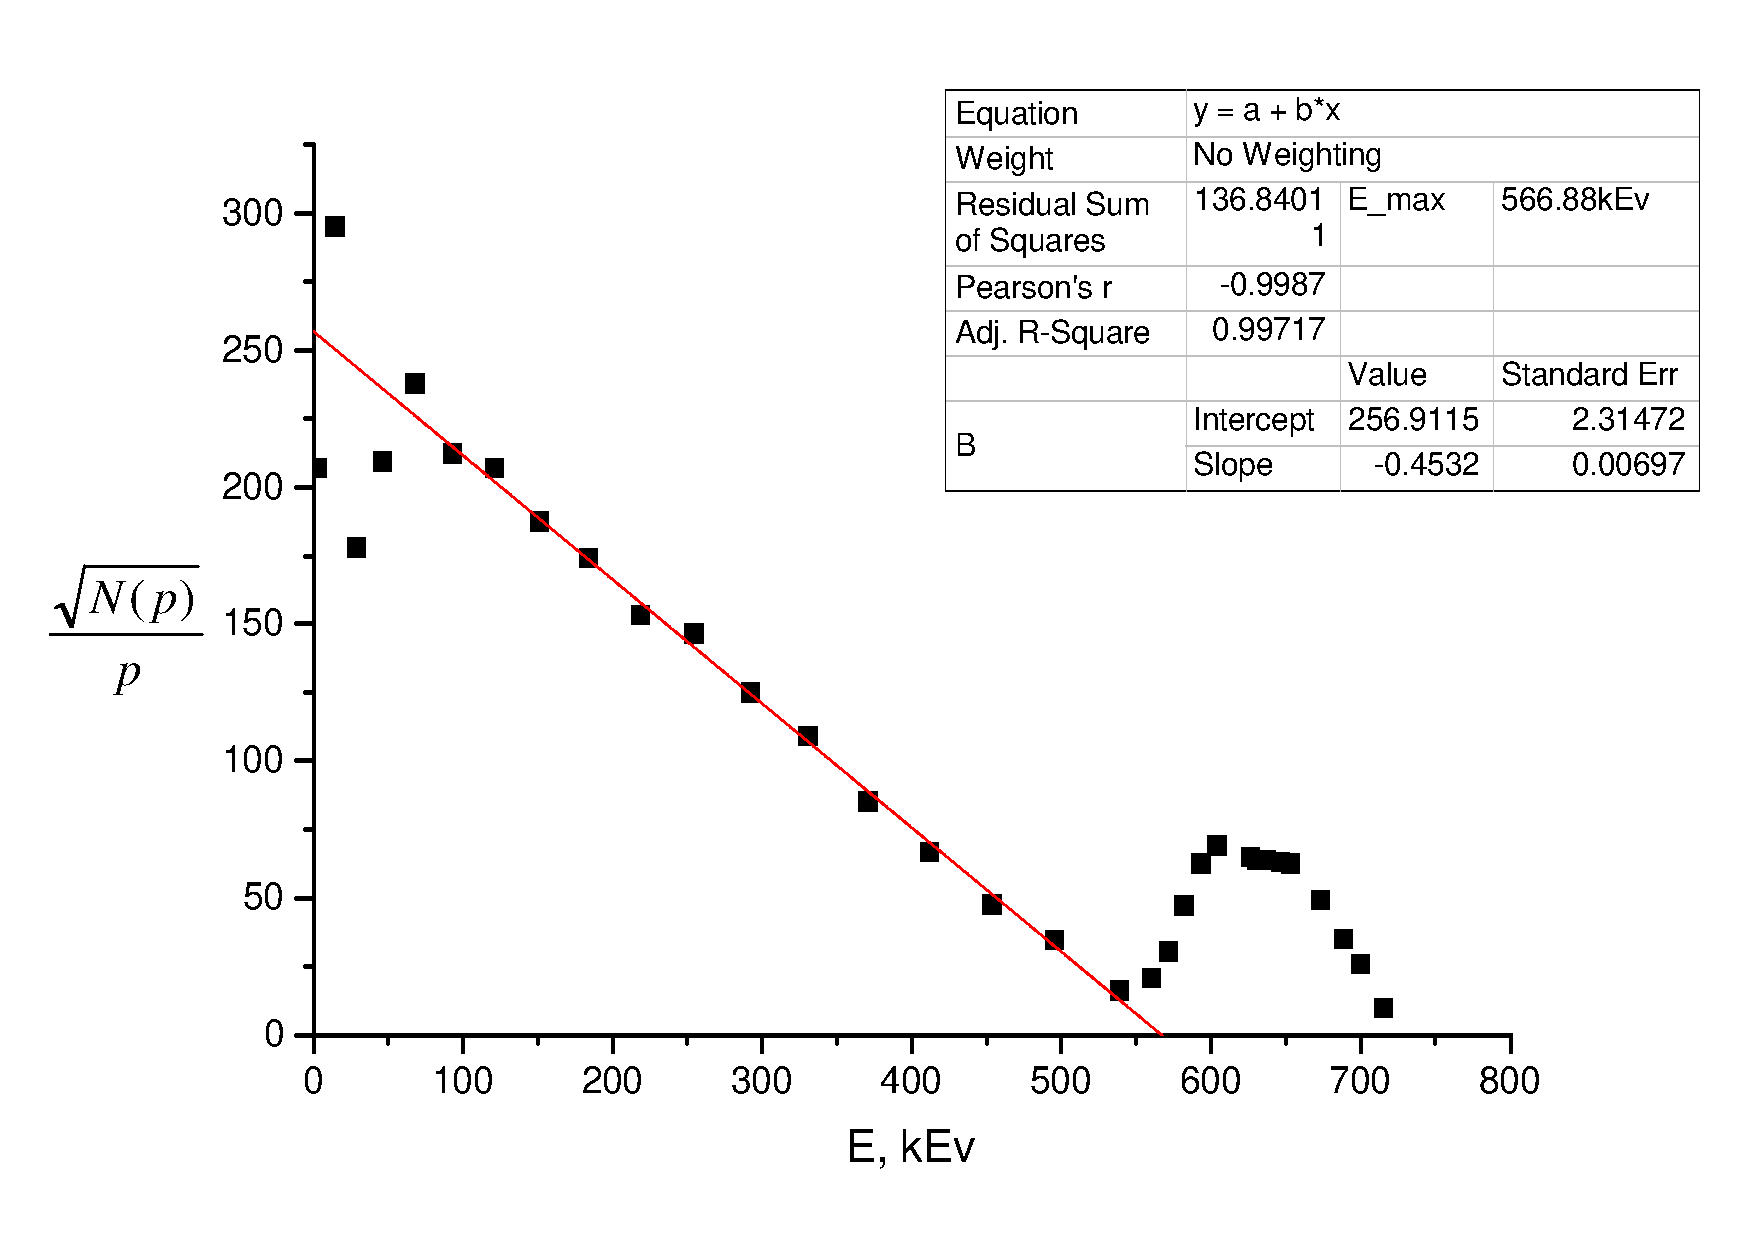
\includegraphics[width=\linewidth]{fermi.pdf}
			\caption{Форма спектра $\beta$-частиц при разрешенных переходах}
		\end{figure}
		
		
По точке пересечения графика с осью абсцисс определим максимальную энергию электронов в $\beta$-спектре. 
$E_{max} = 566.9 kEv$

\newpage

\section{Вывод и обсуждение результатов}
		В проделанной работе было исследовано явление $\beta$-распада $^{137}Cs$. Выяв лен <<полудискретный>> характер спектра: непрерывная часть обеспечивается за счет рождения двух частиц, дискретный пик --- рождение конверсионных электронов.
		Непрерывность спектра доказывает существование антинейтрино и его рождение в процессе $\beta^-$ распада. Также было выяснено существование конверсионных электронов --- частиц, испускаемых в результате перехода ядра на более низкий энергетический уровень. Их энергетический спектр является уже дискретным, т.к. их энергия строго привязана к энергиям жлектронных уровней в атоме.
\end{document}


